\documentclass[xcolor=table,aspectratio=169]{beamer}
\usepackage{beamerthemesplit}
\usepackage{wrapfig}
\usetheme{SPbGU}
\usepackage{pdfpages}
\usepackage{amsmath}
\usepackage{cmap}
\usepackage[T2A]{fontenc}
\usepackage[utf8]{inputenc}
\usepackage[english]{babel}
\usepackage{indentfirst}
\usepackage{mathtools}
\usepackage{tikz}
\usepackage{multirow}
\usepackage[noend]{algpseudocode}
\usepackage{algorithm}
\usepackage{algorithmicx}
\usepackage{fancyvrb}

\usepackage{minted}

\usetikzlibrary{calc}
\usetikzlibrary{shapes,arrows}
\usetikzlibrary{arrows,automata}
\usetikzlibrary{positioning}

\usepackage{fontawesome}

\usetikzlibrary{shapes.callouts}

\usepackage{xparse}

%for [[ ]]
\usepackage{stmaryrd}


\tikzset{
    invisible/.style={opacity=0,text opacity=0},
    visible on/.style={alt=#1{}{invisible}},
    alt/.code args={<#1>#2#3}{%
      \alt<#1>{\pgfkeysalso{#2}}{\pgfkeysalso{#3}} % \pgfkeysalso doesn't change the path
    },
}

\NewDocumentCommand{\mycallout}{r<> O{opacity=0.8,text opacity=1} m m m}{%
\tikz[remember picture, overlay]\node[align=center, fill=cyan!20, text width=#5cm,
#2,visible on=<#1>, rounded corners,
draw,rectangle callout,anchor=pointer,callout relative pointer={(230:1cm)}]
at (#3) {#4};
}

%\newcommand{\tikzmark}[1]{\tikz[overlay,remember picture,baseline=-0.5ex] \node (#1) {};}



\usepackage{tabularx}
\newcolumntype{Y}{>{\raggedleft\arraybackslash}X}

\renewcommand{\thealgorithm}{}

\newtheorem{mytheorem}{Theorem}
\renewcommand{\thealgorithm}{}

\newcommand{\tikzmark}[1]{\tikz[overlay,remember picture] \node (#1) {};}
\def\Put(#1,#2)#3{\leavevmode\makebox(0,0){\put(#1,#2){#3}}}

\newcommand{\ltz}{$< 1$}


\tikzset{
    state/.style={
           rectangle,
           rounded corners,
           draw=black, very thick,
           minimum height=2em,
           inner sep=2pt,
           text centered,
           },
}

\beamertemplatenavigationsymbolsempty

\title[Multiple-Source CFPQ]{Multiple-Source Context-Free Path Querying in Terms of Linear Algebra}
%\subtitle[YaccConstructor]{Parsing techniques for graph analysis}
\institute[JB Research, SPbSU]{
JetBrains Research, Programming Languages and Tools Lab  \\
Saint Petersburg State University
}


\author[Semyon Grigorev]{Arseniy Terekhov, Vlada Pogozhelskaya, Vadim Abzalov, \\ Timur Zinnatulin, \textbf{Semyon Grigorev}}

\date{March 24, 2021}

\begin{document}
{
\begin{frame}[fragile]
  \begin{table}
  \centering
  \begin{tabularx}{\linewidth}{XcX}
    
\includegraphics[height=1.5cm]{pictures/JB_logo_RGB_research_vert.pdf} \hfill
    & \begin{minipage}[t]{0.3\textwidth}\center 
\includegraphics[height=1.5cm]{pictures/EDBT.png} \hfill
      \end{minipage}
    & \hfill 
\includegraphics[height=1.5cm]{pictures/SPbGU_Logo.png}
  \end{tabularx}
  \end{table}
  \titlepage
\end{frame}
}

\begin{frame}[fragile] \frametitle{Formal Language Constrained Path Querying}
      \begin{minipage}[m]{0.45\linewidth}
  \raisebox{-0.5\totalheight}{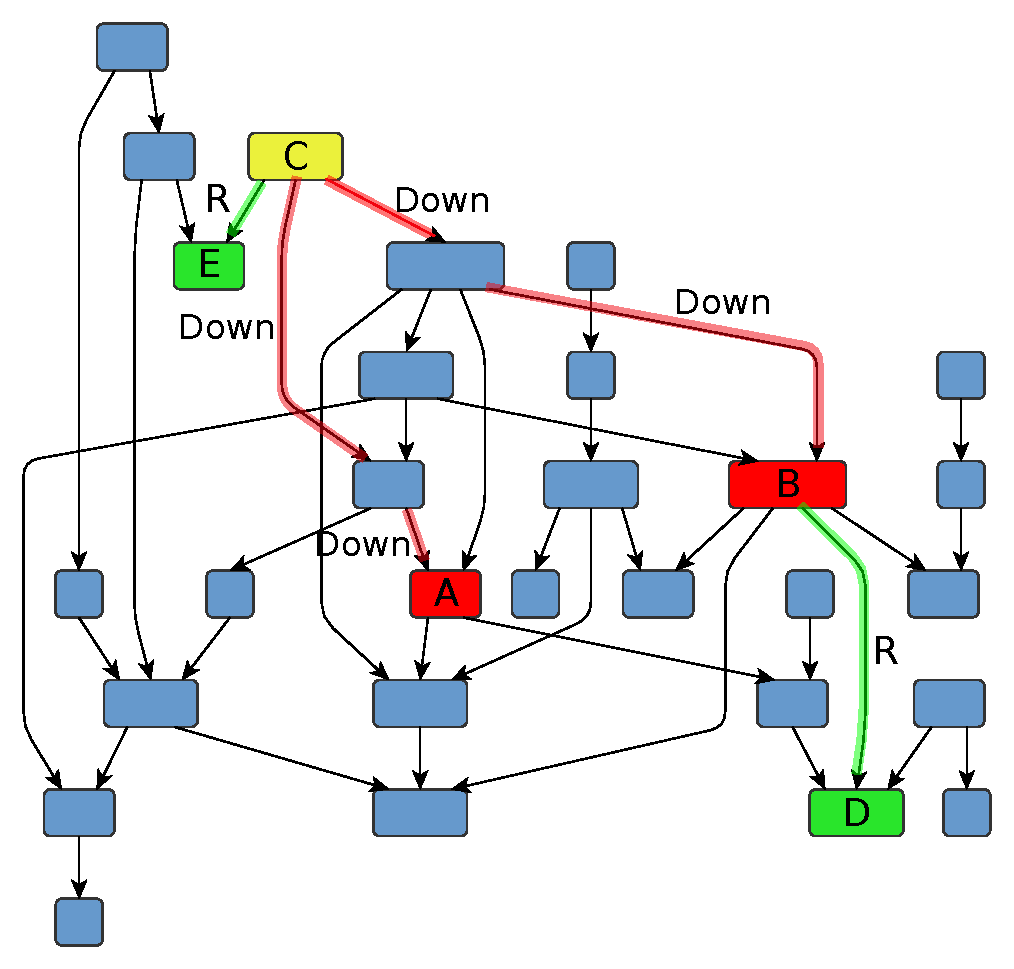
\includegraphics[width=\textwidth]{pictures/hierarchical_rpq.pdf}}
  \end{minipage}\hfill
  \begin{minipage}[m]{0.5\linewidth}
  Navigation through an edge-labeled graph
  \begin{itemize}
        \item \textbf{Path} specifies a \textbf{word} formed by labels of edges
        \item \textbf{Paths constraint} is a \textbf{language}: the path specified word should be in the given language
        \item Constraints expressiveness is related to \textbf{formal languages classes}
  \end{itemize}
  \pause
  Regular path queries (RPQ)
  \begin{itemize}
        \item \textbf{Regular} languages are used as constraints
        \item Which nodes are reachable from \textbf{C} by arbitrary number of $\textbf{R} \text{ and } \textbf{Down}$ edges?
        \item $\mathcal{L} = (\textit{R} \mid \textit{Down})^*$
  \end{itemize}

  \end{minipage}

\end{frame}

\begin{frame}[fragile] \frametitle{Context-Free Path Querying (CFPQ)}
      \begin{minipage}[m]{0.45\linewidth}
  \raisebox{-0.5\totalheight}{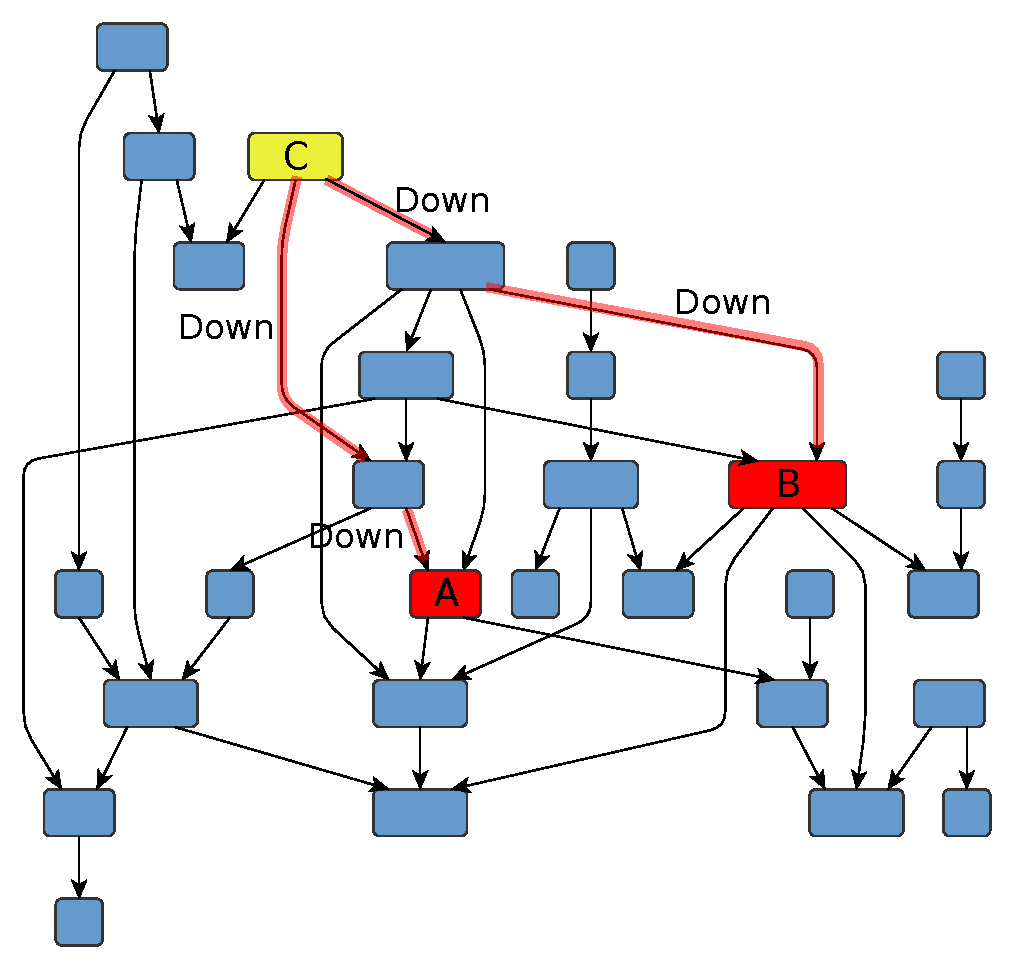
\includegraphics[width=\textwidth]{pictures/hierarchical.pdf}}
  \end{minipage}\hfill
  \begin{minipage}[m]{0.5\linewidth}    
  \begin{itemize}
        \item \textbf{Context-free} languages are used as constraints 
        \item Are nodes A and B on the same level of hierarchy?
        \item Is there a path of form $\overline{\textbf{Down}}^n \, \textbf{Down}^n$ between A and B?
        \item Context-free grammar: $\textit{sameLvl} \to \overline{\textit{Down}} \ \textit{sameLvl} \ \textit{Down} \mid \varepsilon$
  \end{itemize}
  \pause
  Applications
    \begin{itemize}
      \item Static code analysis [\href{https://dl.acm.org/doi/10.1145/199448.199462}{T. Reps, et al, 1995}]
      \item Graph segmentation [\href{https://dblp.org/rec/conf/icde/0001D19.html}{H. Miao, et al, 2019}]
      \item Biological data analysis [\href{https://pubmed.ncbi.nlm.nih.gov/20134073/}{P. Sevon, et al, 2008}]
      \item ...      
    \end{itemize}
    
  \end{minipage}

  \end{frame}

\begin{frame}[fragile] \frametitle{Problem Statement}
%\begin{center}
   There is no support of CFPQ in real-world graph analysis systems (graph databases)
%\end{center}
\pause
   \begin{itemize}     
      \item J. Kuijpers, et al\footnote<.(1)->{Jochem Kuijpers, George Fletcher, Nikolay Yakovets, and Tobias Lindaaker. 2019. An Experimental Study of Context-Free Path Query Evaluation Methods.}: existing algorithms are too slow to be practical (in the context of Neo4j)
      \pause
      \item A. Terekhov, et al\footnote<.(1)->{Arseniy Terekhov, Artyom Khoroshev, Rustam Azimov, and Semyon Grigorev. 2020. Context-Free Path Querying with Single-Path Semantics by Matrix Multiplication.}: linear algebra based CFPQ algorithm can be performant enough
      \pause
      \item There is no full-stack support of CFPQ
      \begin{itemize}
        \item Grammars instead of full-featured queries
        \item Custom graph storage instead of a mature graph database        
      \end{itemize}
    \end{itemize}
  
\end{frame}


\begin{frame}[fragile] \frametitle{Proposed Solution}
  \begin{itemize}
      \item \textbf{Multiple-Source CFPQ} to process only required subset of a graph
      \pause
      \item \textbf{Cypher} extended with \textbf{path patterns}\footnote<.(1)->{Tobias Lindaaker, Path Patterns for Cypher, 2017, \scriptsize \url{https://github.com/thobe/openCypher/blob/rpq/cip/1.accepted/CIP2017-02-06-Path-Patterns.adoc}} to express context-free constraints 
      \pause
      \item \textbf{RedisGraph} database 
      \begin{itemize}
        \item Provides graph storage with matrix-based representation
        \item Contains linear algebra based query engine (SuiteSparse:GraphBLAS\footnote<.(1)->{Timothy A. Davis. 2019. Algorithm 1000: SuiteSparse:GraphBLAS: Graph Algorithms in the Language of Sparse Linear Algebra} is used)
        \item Allows one to use Cypher for querying (libcypher-parser\footnote<.(1)->{Chris Leishman, \url{https://github.com/cleishm/libcypher-parser}} is used)
      \end{itemize}
      
      
  \end{itemize}
  
\end{frame}

\begin{frame}[fragile] \frametitle{Multiple-Source CFPQ}
An improved version of Rustam Azimov CFPQ algorithm\footnote{Rustam Azimov and Semyon Grigorev. 2018. Context-free path querying by matrix multiplication.}
  \begin{itemize}
      \item The set of start vertices can be specified
      \pause
      \item Only required subgraph will be processed      
  \end{itemize}
  
\end{frame}

\begin{frame}[fragile] \frametitle{Multiple-Source CFPQ}
\vspace{-0.5cm}
\tikzmark{zzz}{ }
\small
\begin{algorithmic}[1]
\Function{MultiSrcCFPQ}{$D = (V, E, \Sigma_V, \Sigma_E, \lambda_V, \lambda_E)$, $G=(N,\Sigma,P,S)$, $Src$}
    \State{$T \gets \{T^A \mid  A \in N, T^A[i,j] \gets \textit{false} \text{, for all $i,j$}\} $}

    \State{$TSrc \gets \{TSrc^A \mid  A \in N, TSrc^A[i,j] \gets \textit{false} \text{, for all $i,j$}\}$}

    \ForAll{$ v \in Src$} $TSrc^S[v,v] \gets true$
    \EndFor

    \State $MSrc \gets TSrc^S$

    \ForAll{$A \to x \in P \mid x \in \Sigma_E$} 
        \ForAll{$(v, to) \in E \mid x \in \lambda_E(v,to)$} $T^A[v,to] \gets true$
        \EndFor
    \EndFor

    \ForAll{$A \to x \in P~\mid x \in \Sigma_V$}
        \ForAll{$v \in V~|~ x \in \lambda_V(v)$} $T^A[v,v] \gets true$
        \EndFor
    \EndFor

    \While{$T\ or\ TSrc\ is\ changing$}
        \ForAll{$A \to B C \in P$}
            \State{$M \gets TSrc^A*T^B$}
            \State{$T^A \gets T^A + M*T^C$}
            \State{$TSrc^B \gets TSrc^B + TSrc^A$}
            \State{$TSrc^C \gets TSrc^C + $ \Call{getDst}{$M$}}
        \EndFor
    \EndWhile
    \State \Return $MSrc * T^S$
\EndFunction

\end{algorithmic}


  %}
  \pause
  \onslide<2>{\tikz[overlay,remember picture]{\draw[draw=red,thick,double,fill opacity=0.2] ($ (zzz) + (4.7,-0.1)$) rectangle ($ (zzz) + (13.0,-0.6)$);}}

  \onslide<3>{\tikz[overlay,remember picture]{\draw[draw=red,thick,double,fill opacity=0.2] ($ (zzz) + (0.8,-0.6)$) rectangle ($ (zzz) + (9.8,-4.23)$);}}

  \onslide<4>{\tikz[overlay,remember picture]{\draw[draw=red,thick,double,fill opacity=0.2] ($ (zzz) + (0.8,-4.23)$) rectangle ($ (zzz) + (9.8,-6.76)$);}}

  \onslide<5>{\tikz[overlay,remember picture]{\draw[draw=red,thick,double,fill opacity=0.2] ($ (zzz) + (0.8,-6.76)$) rectangle ($ (zzz) + (9.8,-7.26)$);}}

  %\onslide<5>{\tikz[overlay,remember picture]{\draw[draw=red,thick,double,fill opacity=0.2] ($ (zzz) + (7.8,5.1)$) rectangle ($ (zzz) + (11.8,0.35)$);}}

  %\onslide<6>{\tikz[overlay,remember picture]{\draw[draw=red,thick,double,fill opacity=0.2] ($ (zzz) + (3.9,5.2)$) rectangle ($ (zzz) + (7.8,0.2)$);}}

  %\onslide<7>{\tikz[overlay,remember picture]{\draw[draw=red,thick,double,fill opacity=0.2] ($ (zzz) + (-0.1,4.8)$) rectangle ($ (zzz) + (3.8,4.0)$);}}


%\Function{getDst}{$M$}
%    \State{$A[i,j] \gets \textit{false}$}
%    \ForAll{$(v,to) \in V^2 \mid M[v,to] = true$}
%        \State{$A[to,to] \gets true$}
%    \EndFor
%    \State \Return A
%\EndFunction


\end{frame}


\begin{frame}[fragile] \frametitle{Cypher Extension}
        \begin{minipage}[m]{0.43\linewidth}
  \raisebox{-0.5\totalheight}{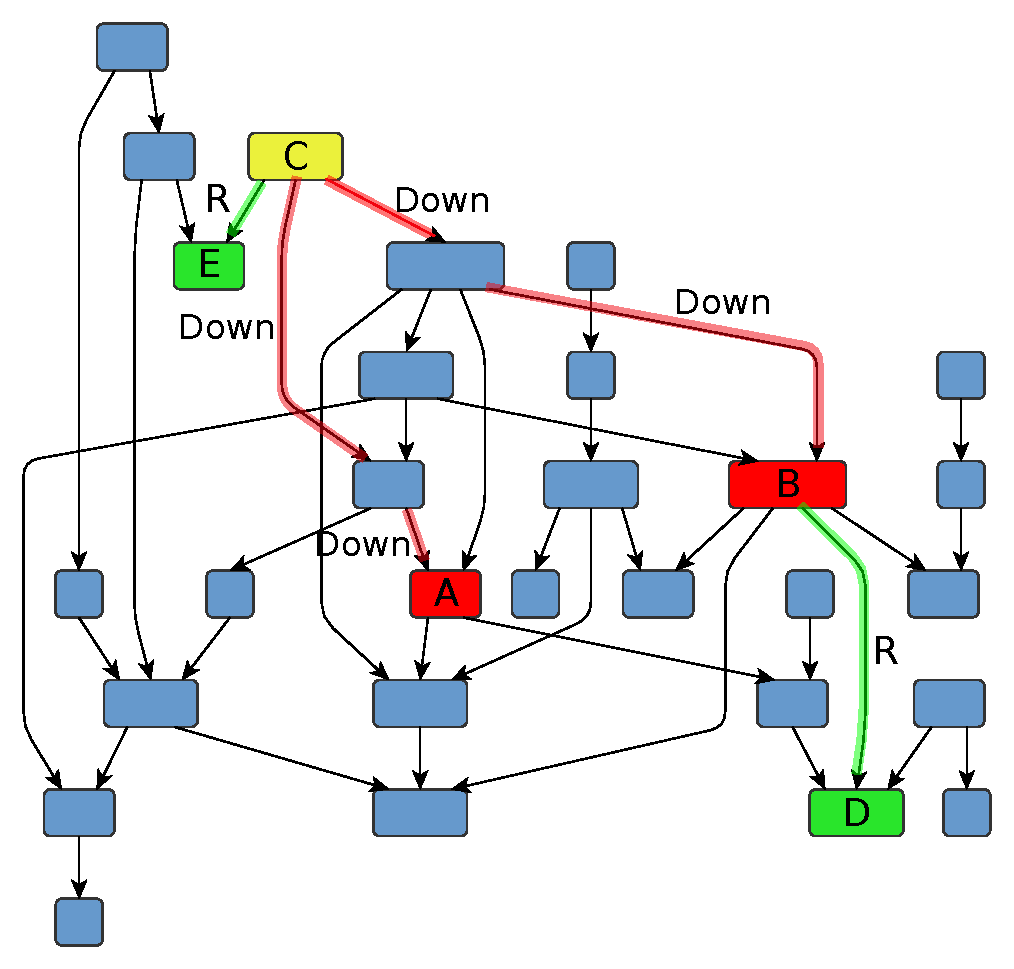
\includegraphics[width=\textwidth]{pictures/hierarchical_rpq.pdf}}
  \end{minipage}\hfill
  \begin{minipage}[m]{0.55\linewidth}
  \begin{minted}{cypher}
MATCH (u)-[(R | Down)*]->(v)
RETURN u.name, v.name
  \end{minted}
  
  \pause
  \vspace{1cm}
  \tikzmark{xxx}{}
  \begin{minted}{cypher}
PATH PATTERN SameLvl = 
  ()-/ <:Down [~SameLvl | ()] :Down> /->()
MATCH (u)-/ ~SameLvl /->(v)
RETURN u.name, v.name
  \end{minted}
  
    {\tikz[overlay,remember picture]{\draw[draw=red, fill opacity=0.2, double, line width=0.25mm] ($ (xxx) + (-0.1,-0.2)$) rectangle ($  (xxx) + (8.6,-1.2)$);}
    \mycallout<2>[opacity=1]{$ (xxx) + (1.15,-0.3)$}{Named path pattern}{3.5}
    %\tikz[overlay,remember picture]{\draw[draw=red, fill opacity=0.2, line width=0.25mm] ($ (xxx) + (8.9,-0.8)$) rectangle ($  (xxx) + (10.8,-1.3)$);}
    \mycallout<2>[opacity=1]{$ (xxx) + (4.9,-1.0)$}{\small $\textit{SameLvl} \to \overline{\textit{Down}} \ \textit{SameLvl} \ \textit{Down} \mid \varepsilon$ }{5.5}
    }


  \end{minipage}


\end{frame}


\begin{frame}[fragile] \frametitle{Implementation Details}
  \begin{itemize}
  \item Linear algebra based multiple-source CFPQ is implemented as a part of RedisGraph query engine
  \item Cypher parser is extended to support path patterns
  \item Path patterns are partially supported\footnote{Full support is a nontrivial challenge: formal description of the extension is required} in RedisGreaph query execution workflow
  \end{itemize}
  
\end{frame}




\begin{frame}[fragile] \frametitle{Evaluation Setup}

\begin{minipage}[t]{0.51\textwidth}
\vspace{-2cm}
\begin{itemize}
  \item Ubuntu 18.04, Intel Core i7-6700 CPU, 3.4GHz, DDR4 64Gb RAM
  \item Graphs stored in RedisGraph with our extensions
  \item Queries are generated with template for given size of start set
  \item The union of all start sets is $V$ 
\end{itemize}

\end{minipage}
\pause
\begin{minipage}[t]{0.44\textwidth}
{
\rowcolors{2}{black!2}{black!10}
\begin{tabular}{|l|c|c|c|}
\hline
Graph                  & \#V                  & \#E                  & Q     \\
              
\hline
\hline
core                   & 1323                 & 4342                 & $g_1$ \\
pathways               & 6238                 & 18 598               & $g_1$ \\
gohierarchy            & 45 007               & 980 218              & $g_1$ \\
enzyme                 & 48 815               & 109 695              & $g_1$ \\
eclass\_514en          & 239 111              & 523 727              & $g_1$ \\
geospecies             & 450 609              & 2 311 461            & $geo$ \\
go                     & 272 770              & 534 311              & $g_1$ \\
\hline
\end{tabular}
}

\end{minipage}

\vspace{1cm}
\pause
\begin{minted}{cypher}
PATH PATTERN S = 
  ()-/ [<:SubClassOf [~S | ()] :SubClassOf] | [<:Type [~S | ()] :Type] /->()
MATCH (src)-/ ~S /->()
WHERE {id_from} <= src.id and src.id <= {id_to}
RETURN count(*)

\end{minted}


\end{frame}

\begin{frame}[fragile] \frametitle{Evaluation Results}  
  \begin{center}
  \begin{minipage}[t]{0.15\textwidth}
  \vspace{1.5cm}
  eclass\_514en\\  
  Query: g1
  \vspace{2.5cm}\\
  geospecies
  Query: geo
  \end{minipage}
  \begin{minipage}[t]{0.4\textwidth}
    \begin{center} 
    %\vspace{-0.5cm}
    Time\\
  \tikzmark{y1}{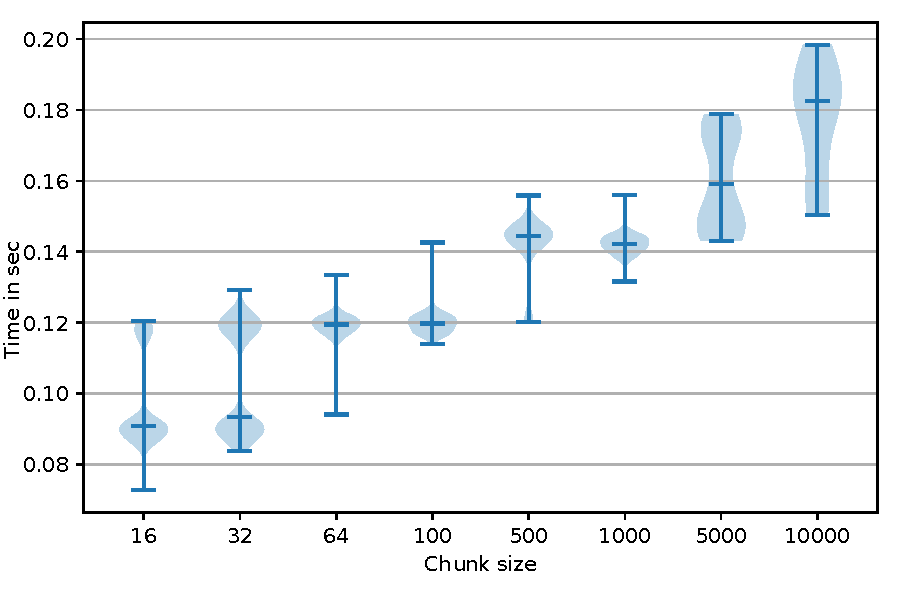
\includegraphics[width=.85\textwidth]{pictures/eclass_514en_time.pdf}}\\
  \tikzmark{y2}{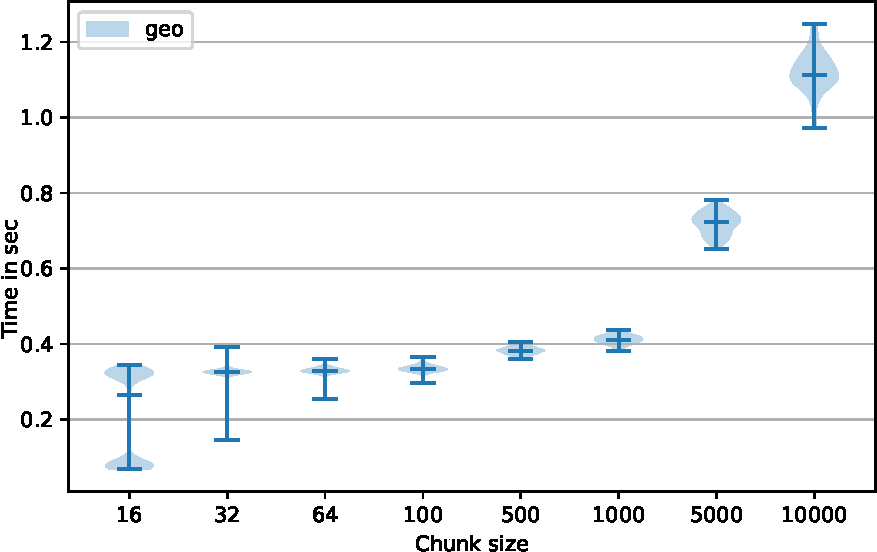
\includegraphics[width=.85\textwidth]{pictures/geospecies_time.pdf}}
\end{center}
\end{minipage}
\begin{minipage}[t]{0.4\textwidth}
  \begin{center}
  %\vspace{-0.5cm}
    Memory\\
  \tikzmark{z1}{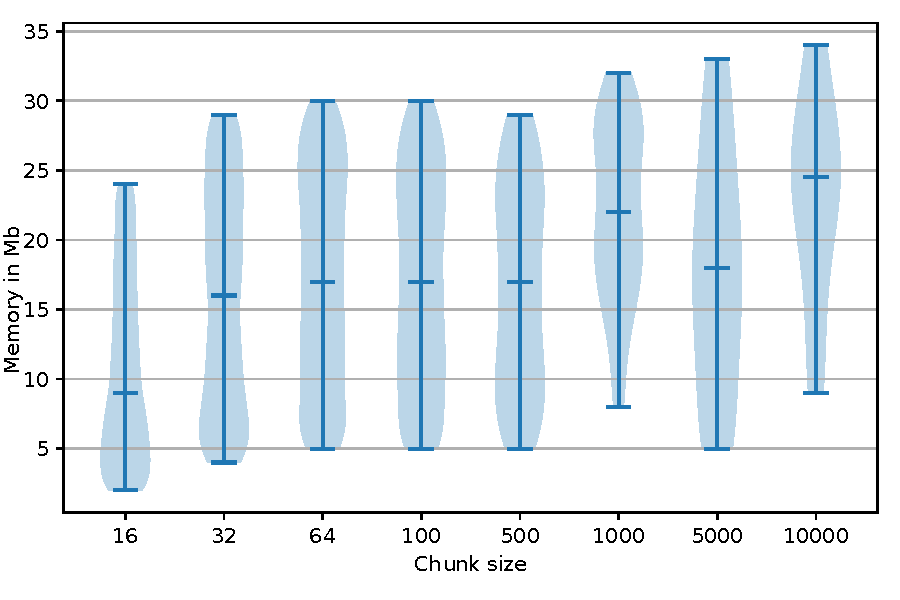
\includegraphics[width=.85\textwidth]{pictures/eclass_514en_mem.pdf}}\\
  \tikzmark{z2}{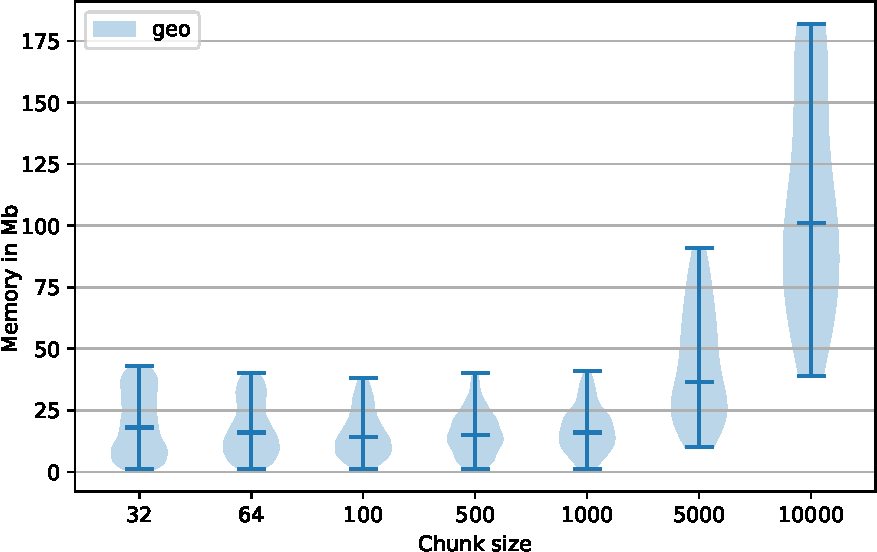
\includegraphics[width=.85\textwidth]{pictures/geospecies_mem.pdf}}
\end{center}
\end{minipage}
\end{center}
\end{frame}


\begin{frame}[fragile] \frametitle{Conclusion}
  \begin{itemize}
      \item Full-stack support for CFPQ in real-world graph query language (Cypher) on the top of real-world graph database (RedisGraph)
      \begin{itemize}
         \item No more context-free grammars
         \item No more custom graph formats and storages
      \end{itemize}
      \item Reasonable performance of context-free path queries
      \begin{itemize}
         \item Multiple-source scenario
         \item Space-time ratio can be tuned
      \end{itemize}
      \item Context-free path queries can be used in applications with well-established tools
  \end{itemize}  
\end{frame}



\begin{frame}[fragile] \frametitle{Future Research}
  \begin{itemize}
    \item Mechanization of Cypher semantics in Coq
    \begin{itemize}
      \item Including path patterns
      \item Correctness of translation to linear algebra
    \end{itemize}
    \pause
    \item Integration of tensor-based CFPQ algorithm\footnote<.(1)->{Egor Orachev, Ilya Epelbaum, R. Azimov and S. Grigorev. “Context-Free Path Querying by Kronecker Product.” ADBIS (2020).} to RedisGraph
    \begin{itemize}
      \item To construct paths, not only reachability facts
      \item The algorithm should be modified to get multiple-source version
    \end{itemize}
    \pause
    \item Detailed evaluation
    \begin{itemize}
      \item More graphs and queries, including RPQs      
      \item Scalability of the solution
      \item Comparison with other graph query engines
    \end{itemize}
  \end{itemize}
\end{frame}

\begin{frame}
\frametitle{Contact Information}
\begin{minipage}[t]{0.8\textwidth}
\begin{itemize}
  \item Try it out (Docker image with extended RedisGraph): \url{https://hub.docker.com/r/simpletondl/redisgraph}
  \item RedisGraph extended with CFPQ: \url{https://github.com/YaccConstructor/RedisGraph}
  \item Cypher parser extended with path patterns: \url{https://github.com/YaccConstructor/libcypher-parser}

  \vspace{0.5cm}  
  \pause
  \item Semyon Grigorev: \href{mailto:s.v.grigoriev@spbu.ru}{s.v.grigoriev@spbu.ru}    
  \item Arseniy Terekhov: \href{mailto:simpletondl@yandex.ru}{simpletondl@yandex.ru}
  \item Vlada Pogozhelskaya: \href{mailto:pogozhelskaya@gmail.com}{pogozhelskaya@gmail.com}
  \item Vadim Abzalov: \href{mailto:vadim.i.abzalov@gmail.com}{vadim.i.abzalov@gmail.com}
  \item Timur Zinnatulin: \href{mailto:teemychteemych@gmail.com}{teemychteemych@gmail.com}
\end{itemize}
\end{minipage}~
\begin{minipage}[t]{0.19\textwidth}
\pause
\vspace{2.5cm}
\center{\huge{Thanks!}}
\end{minipage}
\end{frame}
\end{document}
